\normaltrue
\correctiontrue

%\UPSTIidClasse{11} % 11 sup, 12 spé
%\newcommand{\UPSTIidClasse}{12}

%\section{Rotation simple} %\label{CIN:01:B2:12:01}
\exer{Mouvement R  $\star$ \label{CIN:01:B2:12:02}}
\setcounter{question}{0}\marginnote{\xpComp{CIN}{01}}%\UPSTIcompetence{B2-12}
\index{Compétence B2-12}\index{Compétence CIN-01}
\index{Mécanisme à 1 rotation}
\ifcorrection
\else
\marginnote{\textbf{Pas de corrigé pour cet exercice.}}
\fi

\ifprof
\else
Soit le mécanisme suivant. On a $\vect{AB}=R\vect{i_1}$ avec $R=\SI{20}{mm}$. 
\begin{marginfigure}
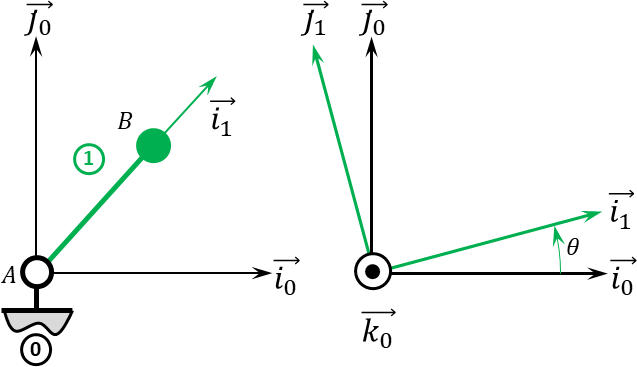
\includegraphics[width=\linewidth]{02_R_01}
\end{marginfigure}
\fi


\question{Tracer le graphe des liaisons.}
\ifprof
\begin{marginfigure}
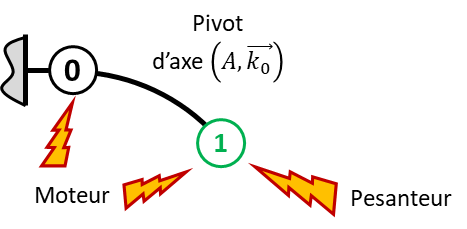
\includegraphics[width=\linewidth]{02_R_01_c}
\end{marginfigure}
\else
\fi

\question{Retracer le schéma cinématique pour $\theta=\dfrac{\pi}{4}\,\text{rad}$.}
\ifprof
\begin{marginfigure}
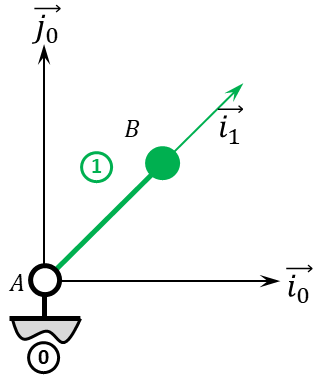
\includegraphics[width=.4\linewidth]{02_R_02_c}
\end{marginfigure}
\else
\fi

\question{Retracer le schéma cinématique pour $\theta={\pi}\, \text{rad}$.}
\ifprof
\begin{marginfigure}
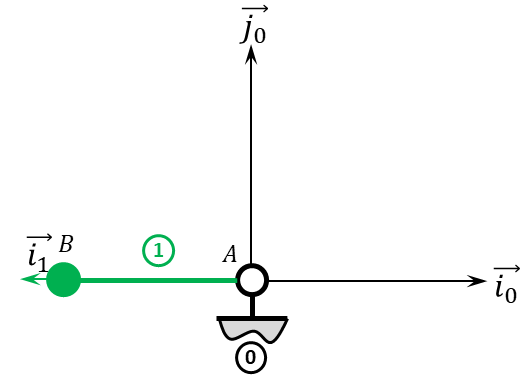
\includegraphics[width=.8\linewidth]{02_R_03_c}
\end{marginfigure}
\else
\fi


\ifprof
\else
\marginnote{Corrigé  voir \ref{CIN:01:B2:12:02}.}
\fi